\documentclass{beamer}
\usepackage[utf8]{inputenc}
\usetheme{Warsaw}%{Berkeley} Madrid
\usecolortheme{Orchid} %dolphin, lily, orchid, structure sidebartab wolverine crane
\title[Conception et adaptation de Serious Games]{Serious games pour la santé :\\ Méthodologie de conception et adaptation de la difficulté}
\author{MÉLIA Geoffrey - Master 2 Informatique}
\institute{Université Montpellier II - NaturalPad}
\date{05 septembre 2013}

\AtBeginSection[]
{
\begin{frame}
\tableofcontents[currentsection,hideallsubsections]
\end{frame}
}

\begin{document}


\begin{frame}
	\titlepage
\end{frame}

%Slide d'intro avant le plan
\begin{frame}{Avant-propos}
	\begin{block}{NaturalPad}
		L'informatique au service de la santé.
	\end{block}		
	\begin{block}{Objectif}
		Adapter la difficulté d'un jeu pour la santé.
	\end{block}		
\end{frame}

%Plan
\begin{frame}{Plan}
	\tableofcontents
\end{frame}

\section{Introduction}
	
	\begin{frame}{NaturalPad}
		\begin{block}{Une SSII dans le secteur de la santé}
			Expert NTIC Santé auprès des Centres Hospitaliers et personnels soignants.\\
			Développeur de serious games à but thérapeutiques.
		\end{block}
		
		\begin{figure}
			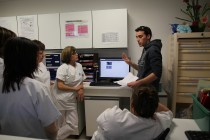
\includegraphics[width=5cm]{../images/formation.jpg}
			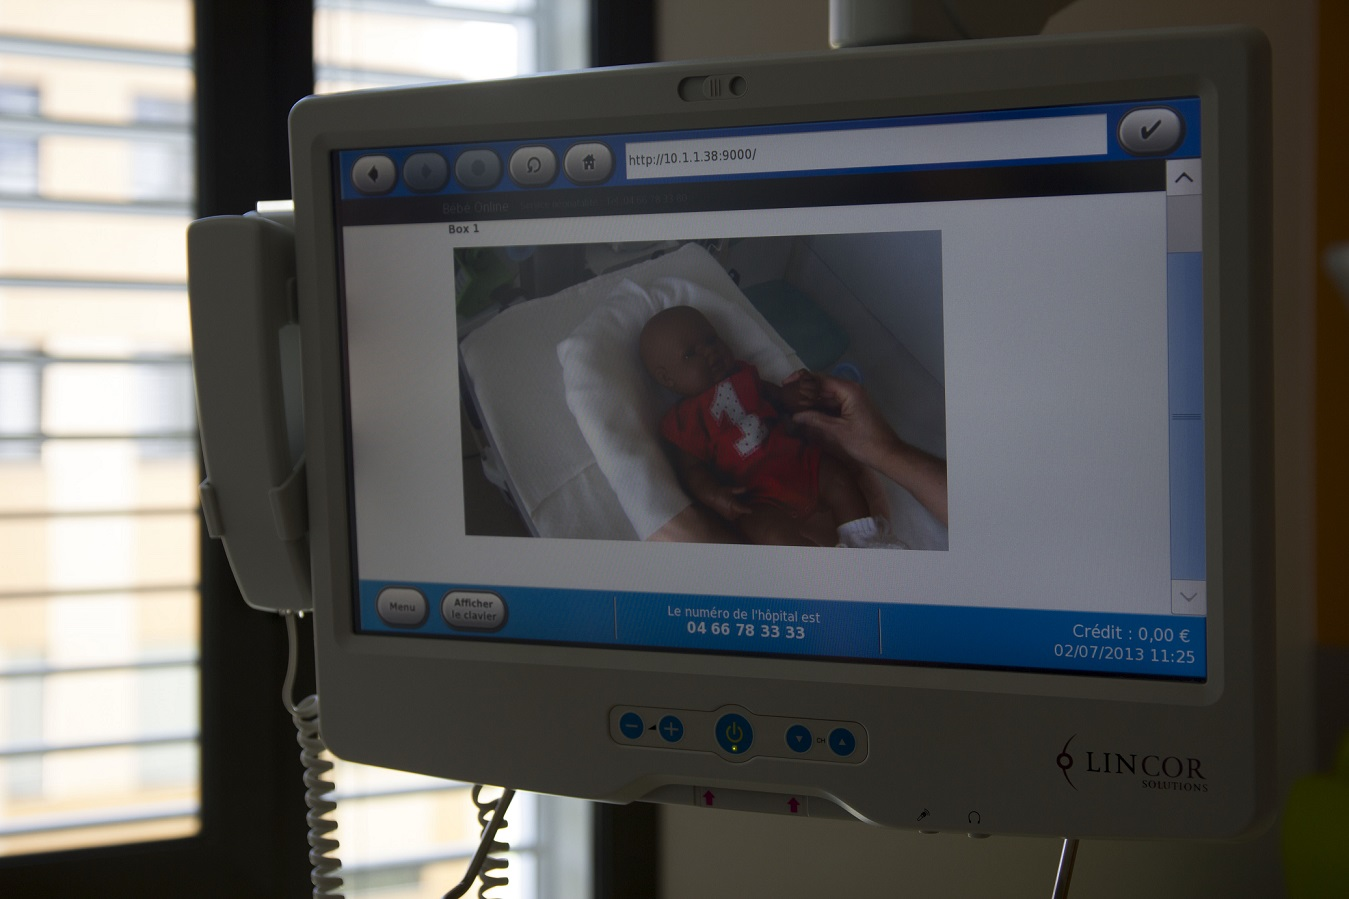
\includegraphics[width=5cm]{../images/bebeonline.jpg}		
			%\caption{A gauche : Formation du personnel médical aux outils déployés. A droite : Terminal avec BebeOnline}	
		\end{figure}
	\end{frame}	

	\begin{frame}{Hammer \& Planks}
		\begin{block}{Un serious game pour la santé}
			• Un jeu vidéo sérieux d'aide à la réhabilitation motrice.\\
			• Adapté aux personnes hémiplégiques : équilibre, membres supérieurs et tronc.
		\end{block}
		
		\begin{figure}
			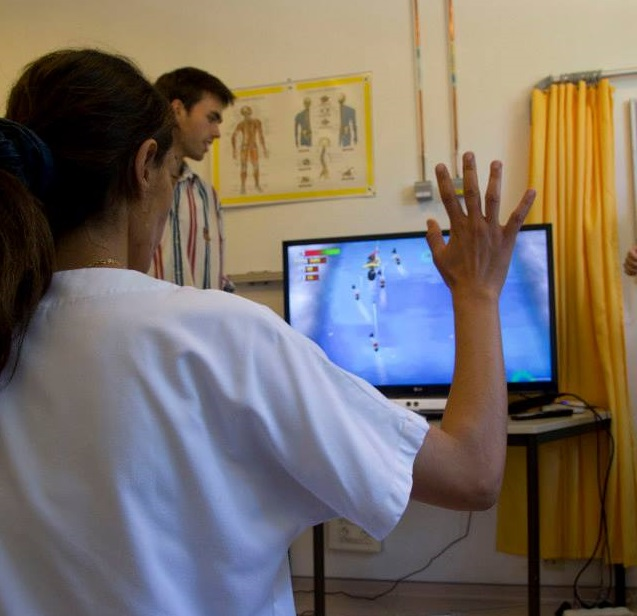
\includegraphics[width=5cm]{../images/test_lapeyronie_2.png}
		\end{figure}
	\end{frame}	
	
	\begin{frame}{Travail d'étude et de recherche : \emph{ZigFugl Meyer}}
		\begin{minipage}{0.40\linewidth}
			\begin{figure}
				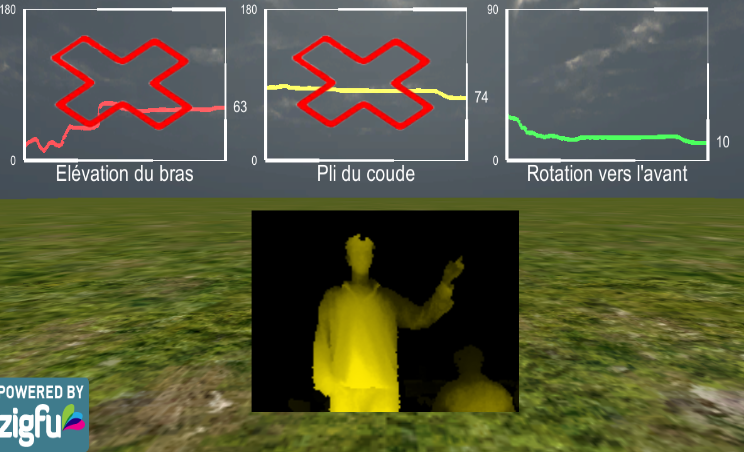
\includegraphics[width=4.2cm]{../images/zigfugl-meyer_1.png}\\
				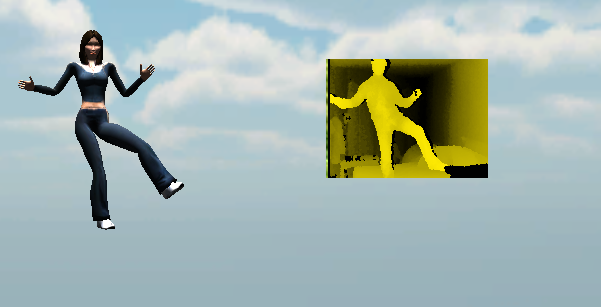
\includegraphics[width=4.2cm]{../images/zigfugl-meyer_2.png}
			\end{figure}
		\end{minipage}
		\begin{minipage}{6cm}%{0.55\linewidth}
			Utilisation de l'informatique pour l'évaluation de capacités motrices (Fugl Meyer assessment). 
				\begin{itemize}
					\item Utilisation de la Kinect comme interface naturelle.
					\item Expérimentation d'une gamification du test.
					\item Vérification automatique de la réussite de l'exercice.
				\end{itemize}
		\end{minipage}
	\end{frame}

\section{Problématique et Objectifs}
	\begin{frame}{Serious Games pour la santé}
		\begin{block}{Utilisation des Serious Games}
			Les jeux
		\end{block}				
	\end{frame}

	\begin{frame}
		\begin{itemize}
			\item Langage utilisé par Beamer: L\uncover<2->{A}TEX
			\item Langage utilisé par Beamer: L\only<2->{A}TEX
		\end{itemize}
	\end{frame}
	
\section{Proposition et réalisations}	
	\begin{frame}
		- interface thérapeutique et ajustement des paramètres
	- méthodo de conception participative
		- conception lombalgie, verticalisation
		- poursuite du travail de TER : fugl meyer informatique
	\end{frame}

\section{Perspectives}
	\begin{frame}
	
	\end{frame}

\section{Conclusion}
	\begin{frame}
	
	\end{frame}

\end{document}